\chapter{Mechanical Waves}

\textit{Life is a wave, which in no two consecutive moments of its existence is composed of the same particles.}\\
\noindent\textbf{-   John Tyndall}

\vspace{1cm}


\begin{marginfigure}%
  \includegraphics[width=\linewidth]{mr_wave.jpg}
  \caption{Portrait of Mr. Wave}
  \label{fig:marginfig}
\end{marginfigure}

\marginnote[30pt]{Mr. Wave (AKA Tony Draughon) was an original member of New York City Breakers.  As an actor he was best known for his performance in the film classic \textit{Beat Street} (1984).  \\ \ \\ \ \\ \ \\
Waving is an illusionary dance style composed of a series of movements that give the appearance that a wave is traversing through a dancer's body.  Waving is thought to have grown out of the popping and funk dance scene.}

\begin{marginfigure}[60pt]
  \includegraphics[width=\linewidth]{the_wave.jpg}
  \caption{Diagram of "The Wave"}
  \label{fig:marginfig}
\end{marginfigure}

\section{Media and Disturbance}
\newthought{A wave is a disturbance}, or oscillation, which propagates through space.  It delivers energy, or information, from one point to another.  We begin to theorize waves considering three criteria for their existence.
\begin{itemize}
\item \textbf{source}\\ A disturbance originates from some region of space at some time.
\item \textbf{medium}\\ The disturbance must propagate through some medium. 
\item \textbf{interaction}\\  For the disturbance to propagate through space there must be some physical means by which adjacent portions of the medium interact in order to pass the disturbance through space.
\end{itemize}
This being said, we may imagine a universe where "in the beginning" waves exist and need not a source.  In addition, the vacuum of empty space may provide the medium for energy to propagate.  A medium is typically considered to be an assembly, or continuum, of "stuff" with inertial properties.  Waves may also travel through nothing. 

\section{Wave Types}

\begin{description}
  \item[transverse wave] A propagating wave that causes the particles of the disturbed medium to move \textbf{perpendicular} to the direction of wave propagation.  "The Wave" at sporting events travels through the crowd as a transverse wave.  
  \item[longitudinal wave] A propagating wave that causes the particles of the disturbed medium to move \textbf{parallel} to the direction of wave propagation.  Sound travels through air as a longitudinal wave.
  
\end{description}

\begin{marginfigure}[0pt]
  \includegraphics[width=\linewidth]{lwav.jpg}
  \caption{Longitudinal wave}
  \label{fig:marginfig}
\end{marginfigure}

\section {One Dimensional Waves}
A wave can take many forms.  In one dimension a wave can be represented by any function of the position plus/minus the product of velocity and time.  The amplitude $A$ represents the maximum value of the function $f(x \pm vt)$.  The wave velocity is the time rate of change of the position on some point of the function $f(x)$.
$$y=f(x-vt) \hspace{2cm} \text{propagation in positive direction}$$
$$y=f(x+vt) \hspace{2cm} \text{propagation in negative direction}$$
$$A=f_{max}$$
$$v=\lim _{\Delta \rightarrow 0}\frac{\Delta x}{\Delta t}=\frac{dx}{dt}=-\frac{\frac{\partial f}{\partial t}}{\frac{\partial f}{\partial x}}$$

\begin{marginfigure}[-130pt]%
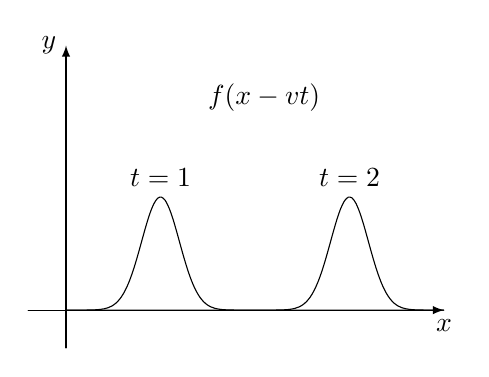
\begin{tikzpicture}
    [line cap=round,line join=round,x=2cm,y=2cm, scale=1.2, decoration={brace,amplitude=2pt}]
 \draw[smooth,samples=100,domain=0:2]
                                 plot(\x,{1.5/(sqrt(2*pi))*exp(-((\x-0.5)^2)/(2*0.1^2))});
 \draw[smooth,samples=100,domain=0:2]
                                 plot(\x,{1.5/(sqrt(2*pi))*exp(-((\x-1.5)^2)/(2*0.1^2))});
   \draw[-latex,color=black,thin] (-0.2,0) -- (2,0) node [anchor=north ,scale=1] {$x$};
   \draw[-latex,color=black,thin] (0,-0.2) -- (0,1.4)node [anchor=east ,scale=1] {$y$};
   \draw (0.7,1) node [anchor=south west ,scale=1] {$f(x-vt)$};
      \draw (0.5,0.6) node [anchor=south ,scale=1] {$t=1$};
   \draw (1.5,0.6) node [anchor=south ,scale=1] {$t=2$};
 \end{tikzpicture}
  \caption{A wave pulse traveling in the positive $x$ direction}
  \label{fig:marginfig}
\end{marginfigure}
 
 \section{Supersposition}
 If two waves are simultaneously propagating through a medium the resultant wave function at any point is the algebraic sum of the wave wave functions of the individual waves.
 
 \section{Waves on Strings (Transverse)}
 \newthought{Consider a wave pulse} traveling along a string with tension $T$ and linear mass density $\mu$.  Zooming in closely to a section of the string the curvature is constant and can therefore be approximated by a circular arc of radius $R$ and angle $\theta$.  \\
The section of string has a net force $F_r$ on it which restores it to equilibrium and a mass $m$.
$$F_r=2F\sin\theta\approx 2F\theta$$
$$m=\mu \Delta s= 2\mu R \theta$$
This force accelerates the section of string centripetally so the velocity of the section of string may be determined as follows.
$$F_r=\frac{mv^2}{R} \hspace{1cm} \longrightarrow \hspace{1cm} 2F\theta=\frac{2\mu R \theta v^2}{R}$$
$$v=\sqrt{\frac{F}{\mu}}$$

\begin{marginfigure}[-220pt]
  \includegraphics[width=\linewidth]{string_wave.jpg}
  \caption{Transverse wave on a string}
  \label{fig:marginfig}
\end{marginfigure}

 \section{Reflection at an Interface}
 
 \begin{itemize}
\item When a wave meets a free boundary, or travels to a less dense/lower velocity medium,  the reflected pulse is not inverted.
\item When a wave meets a fixed boundary, or travels to a more dense/higher velocity medium, the reflected pulse is inverted. 
\end{itemize}

\begin{marginfigure}[0pt]
  \includegraphics[width=\linewidth]{wave_interface.jpg}
  \caption{Transverse wave at an interface (no inversion)}
  \label{fig:marginfig}
\end{marginfigure}

\begin{marginfigure}[0pt]
  \includegraphics[width=\linewidth]{wave_interface2.jpg}
  \caption{Transverse wave at an interface (inversion)}
  \label{fig:marginfig}
\end{marginfigure}

\section{Sinusoidal Waves}
A sinusoidal wave is the smoothest periodic wave.  Here $y$ represents the displacement from equilibrium.  It can represent pressure or a spatial dimension.  $A$ is the amplitude.  It is the maximum $y$ value.  $x$ is the spatial dimension in the direction of propagation.  $t$ is time.  $\phi$ is the phase.  $k$ and $\omega$ are the coefficients of $x$ and $t$ respectively.  
$$y=A\cos\left( kx - \omega t+\phi\right)$$
$k$ and $\omega$ determine the spatial and temporal periodicity.  $\lambda$ is the wavelength and $T$ is referred to as the period.  The wave length is the distance between identical points in the wave.  The period is the time between wave cycles.
$$k\lambda=2\pi \hspace{2cm} \omega T=2\pi$$
The wave speed is defined as the ratio of the wavelength and the period.  It is the speed at which some point on the pattern travels.  It does not represent the speed of any particles in the medium.
$$v_{wave}=\frac{\lambda}{T}=\frac{\omega}{k}$$

\begin{figure}
  \includegraphics[width=\linewidth]{sine_wave.jpg}
  \caption{Sine wave }
  \label{fig:marginfig}
\end{figure}

\subsection{Power}
\marginnote{The power delivered by the wave can be thought of as the rate kinetic energy is delivered in the medium. }
$$\Delta E=\frac{1}{2}(\Delta m)\omega^2A^2=\frac{1}{2}(\mu \Delta x)\omega^2A^2$$
$$P=\frac{\Delta E}{\Delta t}=\frac{1}{2}\mu\omega^2A^2 \frac{\Delta x}{\Delta t}=\frac{1}{2}\mu\omega^2A^2 v_{wave}$$

\newpage

\section{Wave Equation}
Given a scalar function $u(\overrightarrow{\scriptr})$, such as pressure, and propagation speed $c$ we have the following differential equation.  This is known as the wave equation. 
$${\partial^2 u \over \partial t^2} = c^2 \nabla^2 u$$
The functions which obey this differential relationship are waves.  When this differential equation arrises in the analysis of some system it means the systems supports the propagation of waves.

\marginnote{The speed of sound varies with temperature, pressure and the density of the material.  The speed of sound (m/s) in air (at 1 atm) varies with temperature (Celsius) as follows.
$$v=331+0.6T$$}
\section{Sound Waves}
Sound is defined by ANSI as "Oscillation in pressure, stress, particle displacement, particle velocity, etc., propagated in a medium with internal forces (elastic or viscous)."  It can propagate through compressible media such as air, water and solids as longitudinal waves or transverse waves in solids. 
\marginnote{Humans can hear sounds in the range of 20 to 20,000 Hertz, though there is variation between individuals.  Elephants can hear sounds at 14-16hz, while some whales can hear subsonic sounds as low as 7hz (in water).}


The velocity of sound in a medium depends its elastic and inertial properties.
$$v=\sqrt{\frac{\text{elastic property}}{\text{inertial property}}}=\sqrt{\frac{B}{\rho}}$$
\subsection{Power, Intensity and Sound Level}
Consider a sound source emitting energy at a rate $P$.  This is the power of the source.  The intensity of the sound, captured by some observer, is the power per unit area.
$$I=\frac{\text{Power}}{\text{Area}}$$
\begin{marginfigure}[0pt]
  \includegraphics[width=\linewidth]{decibel.jpeg}
  \caption{The decibel scale}
  \label{fig:marginfig}
\end{marginfigure}
The decibel scale of intensity is a logarithmic scale.  The reference value $I_0$ is the lowest intensity of audible sound.
$$\beta=10\  \log \frac{I}{I_0} \hspace{2cm} I_0=10^{-12} \ W/m^2$$

\subsubsection{Spherical, Cylindrical and Linear Waves}
Spherically symmetric waves disperse power over the the surface of a sphere.  Cylindrically symmetric waves disperse power over the the surface of a cylinder.
$$I_{sphere}=\frac{P}{4\pi r^2} \hspace{2cm} I_{cyl}=\frac{P}{2\pi r}$$
Symmetric waves in one dimension give the following intensity.
$$I=\frac{P}{2}$$


\subsection{Doppler Effect}
The Doppler effect is the change in frequency of a wave for an observer moving relative to its source. It is named after the Austrian physicist Christian Doppler, who proposed it in 1842 in Prague. It is commonly heard when a vehicle sounding a siren or horn approaches, passes, and recedes from an observer. Compared to the emitted frequency, the received frequency is higher during the approach, identical at the instant of passing by, and lower during the recession.

$$f = \left ( \frac {c+v_\text{reciever}}{c + v_\text{source}} \right ) f_0$$
\subsection{Standing Waves \& Resonance}
A standing wave is associated with each point on the axis of the wave having an associated constant amplitude. The locations at which the amplitude is minimum are called nodes, and the locations where the amplitude is maximum are called antinodes.

It arises as a result of interference between two waves traveling in opposite directions.  Resonance is the manifestation of standing waves inside a resonator due to interference between waves reflected back and forth at the resonant frequency.
\marginnote{
$$\cos{a}+\cos{b}=2\cos\frac{a+b}{2}\cos\frac{a-b}{2}$$ 
\\ \ \\
$$\sin{a}\pm\sin{b}=2\sin\frac{a\pm b}{2}\cos\frac{a\mp b}{2}$$}

$$A_0\cos(kx-\omega t)+A_0\cos(kx+\omega t)=2A_0 \cos(kx)\cos(\omega t)$$

\subsection{Beats}
A beat is an interference pattern between two sounds of slightly different frequencies, perceived as a periodic variation in volume whose rate is the difference of the two frequencies.  When tuning instruments that can produce sustained tones, beats can readily be recognized. 
$$A_0\cos(\omega_1 t)+A_0\cos(\omega_2 t)=2A_0 \cos(\frac{\omega_1-\omega_2}{2}t)\cos(\frac{\omega_1+\omega_2}{2}t)$$